\chapter{Examples}\label{examples}\index{Examples!of data-sets}
\index{Data!examples}
A large number of examples of the type of calculation that can be run using
MOPAC are supplied with the program.  These examples can be found in the
directory \comp{\ldots/mopac\_examples/}.  Each subdirectory contains data sets
that  illustrate one topic within MOPAC. In order to run any tests, the
contents of the directory should be copied to a new, empty, directory, and the
tests run from this new directory.  Once the tests are complete, the contents
of the new directory can be deleted.  It is important that {\em all} the files
in the  \comp{\ldots/mopac\_examples/} subdirectory be copied.

\section{To verify MOPAC}
\index{port.dat}\index{port.dat}
After MOPAC has been modified, either to make an in-house improvement, or to
port MOPAC to a new platform, you might want to verify that the program has not
been damaged.  Data-set \comp{port.dat} is intended to be used for this
purpose.  This data set makes use of a large fraction (about 85\%) of the code
in MOPAC, and is therefore very sensitive to changes made to the program.
Because it does test most of MOPAC, \comp{port.dat} is very exotic, and does
not represent a realistic calculation.

If the run fails for any reason, the data-set can be edited to remove all the
tests which have been successfully passed, and the new data-set given a new
name.  The new data-set can then be run without having to re-run all the tests
which have been successful.

A test should be considered successful if the criteria on the comment lines
are satisfied.  

The verification data-set also illustrates several of the options within MOPAC,
and may be useful in learning how data-sets are constructed.

Other data sets are included in the examples directory---these test various
options, and are a useful set of templates for designing user specific data
sets.

\section{Excited states}
In order to understand the calculations described in this section, users
should have a good working knowledge of the theory of electronic states.
The example data-set is called \comp{meci.dat}.  This job should be run.
In this discussion, users will be assumed to have access to the output
from \comp{meci.dat}.

\subsection{Discussion of output from \comp{meci.dat}}
\subsubsection{The methyl radical}
Although configuration interaction is primarily used  for calculating excited
states, the first calculation is in fact not an excited state, but a radical,
the methyl radical, CH$_3^.$. This system is used to illustrate a very simple
configuration interaction calculation.  The methyl radical has 7 electrons, 4
from carbon and 1 from each of the three hydrogen atoms.  The lowest three
M.O.s (1a$_{1}'$, at -28.6eV, and  1e$'$ at -14.3eV)  each have two electrons,
followed by a half-filled M.O., (1a$_{2}''$ at -4.1eV)  with only one electron,
then  there are three empty levels (2e$'$ at 5.0eV and 2a$_{1}'$ at 5.3eV).

Only one M.O., the 1a$_{2}''$, is involved in the C.I. In this calculation, 
the energy due to the half-electron approximation is removed, and the energy 
of the pure microstate, in which the odd electron is given $\alpha$ spin, is 
calculated.  Since only one configuration is involved, this new energy is the
energy of the pure state {\em relative to the energy of the system calculated
using half an $\alpha$ and half a $\beta$ electron}.  This amounts to -2.77eV. 
The energy of a methyl radical is then equal to the SCF energy, 89.7~kcal/mol,
plus the C.I.\ energy, -2.77eV (=-63.9~kcal/mol) = 25.8~kcal/mol.

The symmetry of the state is $^2$A$_{2}''$.

\subsubsection{Oxygen}
Molecular oxygen contains 12 valence electrons, with two unpaired electrons in
a $\pi_g$ M.O.  In order to preserve symmetry, $\mathrm{D}_{\infty h}$, the SCF must be
carried out with one electron in each of the two degenerate $\pi_g$ M.O.s. To
allow for this, \comp{OPEN(2,2)} is used.   The energy of the ground-state is
-6.15eV relative to the SCF energy of 126.4~kcal/mol.  This means that the
predicted energy of $^3\Sigma_g^-$ molecular oxygen is -15.4~kcal/mol. 

Because \comp{TRIPLET} was specified, the microstate chosen has an M$_S$=1; in
other words, both electrons in the active space were of $\alpha$ spin. As a
result, the spin density can be calculated using \comp{ESR}, and this gives
exactly 1.0 unpaired electrons in the $p-\pi$ atomic orbitals.  

When specifying \comp{TRIPLET}, information regarding the other states is not
calculated.  These other states can be calculated by simply eliminating
\comp{TRIPLET}.  When this is done, we see that the triplet state is, indeed,
the ground state, but now two other states, excited states, are also
generated.  These are the $^1\Delta_g$ and $^1\Sigma_g$ states at 0.79eV and
1.59eV above the ground state, respectively.

The choice of  M$_S$ can be over-ridden if \comp{ M$_S$} is used.  By
specifying  \comp{M$_S$=0} and \comp{TRIPLET}, all the states are generated,
although only the triplet state would be used in determining which state was to
be selected.

\subsubsection{Methane}
In this calculation, methane is specified, and an \comp{OPEN(6,3)} is used.
Normally, \comp{OPEN(n$_1$,n$_2$)} implies a C.I.\ calculation, but since
the result is obvious (A C.I.\ on a simple closed-shell system involving
only one microstate does exactly nothing.), C.I.\ is not used.
\subsubsection{Methane Cation}
Now, with 5 electrons in a three-fold degenerate t$_2$ M.O., three microstates
are involved in the C.I. These microstates form a degenerate $^2$T$_2$ state.

In earlier MOPACs, systems with degenerate states could not be optimized.  Such
systems would undergo Jahn-Teller distortion, and the degeneracy would be lost.
Starting with MOPAC~93, such states could be optimized (see Section~\ref{dest}).
Several other open shell calculations are given in \comp{meci.dat}; these
illustrate various types of configuration interaction calculations.

\section{Simple geometry optimization}  
The data-set for a simple system is shown in Figure~\ref{ch2o1}.  The old MOPAC
format is used here, so keyword \comp{MOPAC} must be used, otherwise the first
hydrogen atom would be positioned at Cartesian coordinate (1.1,120.0,0).

\begin{figure}
\begin{makeimage}
\end{makeimage}
\begin{verbatim}
Line  1:  MOPAC SYMMETRY
Line  2:  Formaldehyde, for Demonstration Purposes
Line  3:
Line  4:   O
Line  5:   C 1.2 1
Line  6:   H 1.1 1 120 1
Line  7:   H 1.1 0 120 0 180 0 2 1 3 
Line  8:
Line  9:   3 1 4
Line 10:   3 2 4
Line 11:
\end{verbatim}
\begin{center}
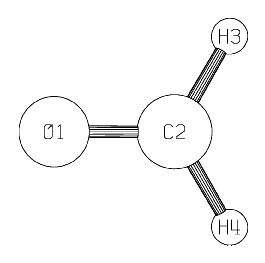
\includegraphics{picch2o}
\end{center}
\caption{\label{ch2o1}Example of a Simple Geometry Optimization}
\index{Formaldehyde, data set}
\end{figure}

These data could be more neatly written as shown in Figure~\ref{ch2o2}.
Now the new coordinate convention is used---the position of the first 
hydrogen is defined in terms of atoms 1 and 2.
\begin{figure}
\begin{makeimage}
\end{makeimage}
\begin{verbatim}
Line  1:  SYMMETRY
Line  2:  Formaldehyde, for Demonstration Purposes
Line  3:
Line  4:   O
Line  5:   C   1.20 1     0.00 0     0.00 0  1
Line  6:   H   1.10 1   120.00 1     0.00 0  2 1
Line  7:   H   1.10 0   120.00 0   180.00 0  2 1 3
Line  8:
Line  9:   3,  1,  4,
Line 10:   3,  2,  4,
Line 11:
\end{verbatim}
\caption{\label{ch2o2} Example of a Simple Geometry Optimization (2)}
\end{figure}
      
These two data-files will produce identical results files.
\begin{figure}
\begin{makeimage}
\end{makeimage}
\compresstable
\begin{verbatim}
  MOPAC CHARGE=2 OPEN(4,3) SINGLET ROOT=6 FORCE
  Methane RHF dication, 6th singlet state (totally symmetric)
  Check that vibrational frequencies are 1338(T2) 2482(A1) 2551(E) 4616(T2) +/-1
   H
   C   1.2298156
   H   1.2298156 0   109.471221
   H   1.2298156 0   109.471221 0  -120.000000 0   2 1 3
   H   1.2298156 0   109.471221 0   120.000000 0   2 1 3
\end{verbatim}
\caption{\label{ech4}Example of an Electronic Excited State}
\end{figure}

\section{Highly excited methane dication}
\index{Methane, data set}
\index{Excited electronic state}
\index{OPEN!use of}
\index{ROOT!use of}
\index{FORCE!use of}
\index{CHARGE!use of}

In this calculation we see that the vibrational frequencies of a highly excited
state can be easily calculated. 

The system being studied is CH$_4^{++}$, in the A$_1$ electronic state. The
t$_2$ level, which normally holds six electrons, has lost two, and therefore
has an occupancy of 4/3 electrons per M.O.  These 4 electrons in 3 levels give
rise to 9 microstates.  The 6th singlet state is non-degenerate, and is the one
chosen for the \comp{FORCE} calculation.  This completes the description of the
calculation.  All that remains is to generate the data-set; this is presented
in Figure~\ref{ech4}.

\section{Polytetrahydrofuran}
The data set shown in Figure~\ref{pthf} illustrates the data file for a 
polytetrahydrofuran\index{Data!for polytetrahydrofuran} calculation. As you can
see the layout of the data is almost the same as that for a molecule, the main 
difference being the presence of the translation vector atom ``Tv''. This data
set would allow calculation of all polymer properties {\em except} band
structure and density of states.  The reason why these properties could not be
calculated is that the polymer units are not correctly specified. In order for
the band-structure to be calculated, the order in which each atom in every mer
occurs must be exactly the same.  An example of such a  numbering system is
given for polyethylene, Figure~\ref{polyc2h4}.

\begin{figure}
\begin{makeimage}
\end{makeimage}
\compresstable
\begin{verbatim}
  Line 1 : T=4H  F
  Line 2 : POLY-TETRAHYDROFURAN (C4 H8 O)2
  Line 3 :
  Line 4a:   C   0.000000 0     0.000000 0     0.000000 0  0 0 0
  Line 4b:   C   1.551261 1     0.000000 0     0.000000 0  1 0 0
  Line 4c:   O   1.401861 1   108.919034 1     0.000000 0  2 1 0
  Line 4d:   C   1.401958 1   119.302489 1   179.392581 1  3 2 1
  Line 4e:   C   1.551074 1   108.956238 1   179.014664 1  4 3 2
  Line 4f:   C   1.541928 1   113.074843 1   179.724877 1  5 4 3
  Line 4g:   C   1.551502 1   113.039652 1   179.525806 1  6 5 4
  Line 4h:   O   1.402677 1   108.663575 1   179.855864 1  7 6 5
  Line 4i:   C   1.402671 1   119.250433 1  -179.637345 1  8 7 6
  Line 4j:   C   1.552020 1   108.665746 1  -179.161900 1  9 8 7
  Line 4k:  XX   1.552507 1   112.659354 1  -178.914985 1 10 9 8
  Line 4l:  XX   1.547723 1   113.375266 1  -179.924995 1 1110 9
  Line 4m:   H   1.114250 1    89.824605 1   126.911018 1  1 3 2
  Line 4n:   H   1.114708 1    89.909148 1  -126.650667 1  1 3 2
  Line 4o:   H   1.123297 1    93.602831 1   127.182594 1  2 4 3
  Line 4p:   H   1.123640 1    93.853406 1  -126.320187 1  2 4 3
  Line 4q:   H   1.123549 1    90.682924 1   126.763659 1  4 6 5
  Line 4r:   H   1.123417 1    90.679889 1  -127.033695 1  4 6 5
  Line 4s:   H   1.114352 1    90.239157 1   126.447043 1  5 7 6
  Line 4t:   H   1.114462 1    89.842852 1  -127.140168 1  5 7 6
  Line 4u:   H   1.114340 1    89.831790 1   126.653999 1  6 8 7
  Line 4v:   H   1.114433 1    89.753913 1  -126.926618 1  6 8 7
  Line 4w:   H   1.123126 1    93.644744 1   127.030541 1  7 9 8
  Line 4x:   H   1.123225 1    93.880969 1  -126.380511 1  7 9 8
  Line 4y:   H   1.123328 1    90.261019 1   127.815464 1  91110
  Line 4z:   H   1.123227 1    91.051403 1  -125.914234 1  91110
  Line 4A:   H   1.113970 1    90.374545 1   126.799259 1 101211
  Line 4B:   H   1.114347 1    90.255788 1  -126.709810 1 101211
  Line 4C:  Tv  12.299490 1     0.000000 0     0.000000 0  11110
  Line 5 :   0   0.000000 0     0.000000 0     0.000000 0  0 0 0
\end{verbatim}
\caption{\label{pthf}Example of a One-Dimensional Polymer}
\index{Polymers!example}  
\index{Polytetrahydrofuran}
\end{figure}

Polytetrahydrofuran has a repeat unit of $\chem (C_4H_8O)_2$: i.e., twice  the 
monomer  unit.   This is necessary in order to allow the lattice to repeat
after a translation through $12.3$~\AA.   See Section~\ref{solid-state} on
Solid State Capability for further details.

Note the two dummy atoms on lines 4k and 4l.  These are useful, but not
essential, for defining the geometry.  The atoms on lines 4y to 4B use these
dummy atoms, as does the translation vector on  line 4C.    The  translation 
vector  has  only  the  length  marked  for optimization.

\begin{figure}
\begin{makeimage}
\end{makeimage}
\begin{center}
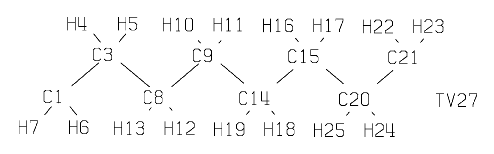
\includegraphics{picpolyc2h4}
\end{center}
\compresstable
\begin{verbatim}
 SYMMETRY MERS=4
 Polyethylene

  C    0.00 0      0.0 0      0.0 0    0  0  0
 XX    7.73 1      0.0 0      0.0 0    1  0  0
  C    1.50 1      0.0 0      0.0 0    1  2  0
  H    1.10 1    109.0 1      0.0 1    3  1  2
  H    1.10 0    109.0 0    120.0 1    3  1  4
  H    1.10 0    109.0 0    180.0 1    1  2  4
  H    1.10 0    109.0 0     60.0 1    1  2  4
  C    1.54 1    110.2 1     60.0 0    3  1  6
  C    1.50 0    110.2 0    180.0 0    8  3  1
  H    1.10 0    109.0 0    -60.0 0    9  8  3
  H    1.10 0    109.0 0     60.0 0    9  8  3
  H    1.10 0    109.3 1    -60.1 1    8  3  1
  H    1.10 0    109.3 0     60.1 0    8  3  1
  C    1.54 0    110.2 0    179.9 0    9  8  3
  C    1.50 0    110.2 0    180.0 0   14  9  8
  H    1.10 0    109.0 0    -60.0 0   15 14  9
  H    1.10 0    109.0 0     60.0 0   15 14  9
  H    1.10 0    109.3 0    -60.1 0   14  9  8
  H    1.10 0    109.3 0     60.1 0   14  9  8
  C    1.54 0    110.2 0    180.0 0   15 14  9
  C    1.50 0    110.2 0    180.0 0   20 15 14
  H    1.10 0    109.0 0    -60.0 0   21 20 15
  H    1.10 0    109.0 0     60.0 0   21 20 15
  H    1.10 0    109.3 0    -60.1 0   20 15 14
  H    1.10 0    109.3 0     60.1 0   20 15 14
 XX    1.54 0    110.2 0    179.9 0   21 20 15
 Tv   10.00 1      0.0 0      0.0 0    1 26  2
\end{verbatim}

\begin{verbatim}
  3  1  9 15 21
  4  1  5  6  7 10 11 12 13 16 17 18 19 22 23 24 25
  4  2  5  6  7 10 11 16 17 22 23
  6  3  9 15 20 21
  6 14 14 26
  7  3  8 11 17 23
  7 14 10 16 22
  8  1 14 20 26
  8  2  9 14 15 20 21 26
 12  2 13 18 19 24 25
 12  3 18 24
 12 14 13 19 25
\end{verbatim}
\caption{\label{polyc2h4}Example of the use of \comp{MERS}}
\index{Polyethylene}\index{MERS!use of}\index{EF!use of}
\end{figure}

\section{Diamond}
\index{Diamond!data for}\index{Data!for diamond|ff}
Data sets for solids are very complicated, and should only be made using
the program MAKPOL.  For diamond, the data-set used by MAKPOL to make the
diamond lattice can be found in Figure~\ref{makpolc}.  The full data set for
diamond is quite large.  Part of this data set is shown in Figure~\ref{c64}.
\index{BCC!use of}
\begin{figure}
\begin{makeimage}
\end{makeimage}
\compresstable
\begin{verbatim}
 MERS=(4,4,4) BCC PM3   1SCF GRADIENTS  PL PRECISE
 Diamond, 64 atoms
 
  C    0.00000000 0    0.0000000 0    0.0000000 0    0  0  0
  C    1.54478440 1    0.0000000 0    0.0000000 0    1  0  0
  C    2.95803659 1  100.0249853 1    0.0000000 0    2  1  0
  C    1.54478440 0  100.0249853 0 -179.9999981 1    3  2  1
  C    1.54478419 0  109.4712159 1  -59.9999996 1    2  1  3
  C    1.54478440 0  109.4712162 0 -179.9999988 0    5  2  1
  C    1.54478417 0  109.4712193 0  120.0000002 1    4  3  2
  C    1.54478440 0  109.4712186 0  180.0000000 0    7  4  3
  C    2.52262210 1   90.0000000 1  -90.0000000 1    5  2  1
  C    1.54478436 0   90.0000010 0 -109.4712164 1    9  5  2

  (Many lines missing)

  C    1.54478398  0  109.4712072  0 -179.9999979  0   38   37   18
  C    1.54478440  0  109.4711954  0  179.9999991  0   57   38   37
  C    1.54478338  0  109.4711915  0  179.9999966  0   40   39   20
  C    1.54478440  0  109.4711797  0  179.9999988  0   59   40   39
  C    1.54478408  0  109.4712137  0  180.0000000  0   42   41   22
  C    1.54478463  0  109.4712020  0  179.9999991  0   61   42   41
  C    1.54478352  0  109.4711940  0  179.9999991  0   44   43   24
  C    1.54478440  0  109.4711782  0  179.9999985  0   63   44   43
 XX    2.52262206  0   90.0000020  0   89.9999974  0    7    4    3
 XX    2.52262208  0   90.0000018  0   90.0000001  0   29   10    9
 XX    2.52262210  0   89.9999999  0  -90.0000008  0   53   34   33
 Tv    7.13505280  1    0.0000000  0    0.0000000  0    1   65    2
 Tv    7.13505280  0    0.0000000  0    0.0000000  0    1   66    2
 Tv    7.13505280  0    0.0000000  0    0.0000000  0    1   67    2
\end{verbatim}

This data set was generated by MAKPOL acting on \comp{make\_diamond.dat}.
Contents of \comp{make\_diamond.dat}:

\begin{verbatim}
 MERS=(4,4,4) BCC PM3   1SCF GRADIENTS  PL PRECISE
 Diamond, 64 atoms

 c
 xx 0.7723922 1
 c  0.7723922 0 180 0
 xx 1.0000000 0 54.73561 0   0 0      1 2 3
 xx 1.0000000 0 54.73561 0 120 0      1 2 4
 xx 1.0000000 0 54.73561 0 240 0      1 2 4
 TV 1.7837632 1  0.0     0   0 0      1 4 2
 TV 1.7837632 1  0.0     0   0 0      1 5 2
 TV 1.7837632 1  0.0     0   0 0      1 6 2
\end{verbatim}
\caption{\label{c64}Example of a Three-Dimensional Data-set}
\end{figure}

